% Data augmentation
%   Image rotation, zoom, shifting, mirroring
%   Could actually be own section as shared between both models?

% Model walkthrough
%   Final model shape (layer count, params)
%   Hyper-params (and potentially tuning?)
%   Model used (ResNet50) - why?
%   approaches to reduce over-fitting (drop-out, regularisation (still need to add))
%   approaches to reduce vanishing gradients (additive layers)
%   approaches to vanishing weights (leaky-relu)
%   FCN layers (different to model A?)
%   probs not image of graph (as massive), but can add to appendix


% Training and learning
%   Time to train, etc
%   Learning curves

% Link to colab notebook


% Some Data
% Epoch 18/50
% 125/125 [==============================] - 47s 374ms/step - loss: 122.8190 - age_output_loss: 105.4552 - gender_output_loss: 0.1736 - age_output_mean_absolute_error: 7.4054 - gender_output_binary_accuracy: 0.9243 - val_loss: 121.7092 - val_age_output_loss: 93.0191 - val_gender_output_loss: 0.2869 - val_age_output_mean_absolute_error: 7.0714 - val_gender_output_binary_accuracy: 0.8831
% Epoch 19/50
% 125/125 [==============================] - 48s 382ms/step - loss: 117.9897 - age_output_loss: 102.1514 - gender_output_loss: 0.1584 - age_output_mean_absolute_error: 7.3246 - gender_output_binary_accuracy: 0.9315 - val_loss: 117.9857 - val_age_output_loss: 89.8029 - val_gender_output_loss: 0.2818 - val_age_output_mean_absolute_error: 6.6650 - val_gender_output_binary_accuracy: 0.8841
% Epoch 20/50
% 125/125 [==============================] - 46s 367ms/step - loss: 111.8711 - age_output_loss: 96.3492 - gender_output_loss: 0.1552 - age_output_mean_absolute_error: 7.0517 - gender_output_binary_accuracy: 0.9380 - val_loss: 139.8109 - val_age_output_loss: 101.6454 - val_gender_output_loss: 0.3817 - val_age_output_mean_absolute_error: 7.1164 - val_gender_output_binary_accuracy: 0.8599
% Epoch 21/50
% 125/125 [==============================] - 46s 368ms/step - loss: 112.9045 - age_output_loss: 97.3385 - gender_output_loss: 0.1557 - age_output_mean_absolute_error: 7.0633 - gender_output_binary_accuracy: 0.9417 - val_loss: 143.0258 - val_age_output_loss: 112.8344 - val_gender_output_loss: 0.3019 - val_age_output_mean_absolute_error: 7.4501 - val_gender_output_binary_accuracy: 0.8760
% Epoch 22/50
% 125/125 [==============================] - 46s 365ms/step - loss: 111.8078 - age_output_loss: 98.6689 - gender_output_loss: 0.1314 - age_output_mean_absolute_error: 7.0413 - gender_output_binary_accuracy: 0.9455 - val_loss: 119.0313 - val_age_output_loss: 90.8313 - val_gender_output_loss: 0.2820 - val_age_output_mean_absolute_error: 6.6158 - val_gender_output_binary_accuracy: 0.8982
% Epoch 23/50
% 125/125 [==============================] - 47s 371ms/step - loss: 106.3928 - age_output_loss: 93.4850 - gender_output_loss: 0.1291 - age_output_mean_absolute_error: 6.9812 - gender_output_binary_accuracy: 0.9488 - val_loss: 140.9203 - val_age_output_loss: 112.3616 - val_gender_output_loss: 0.2856 - val_age_output_mean_absolute_error: 7.3017 - val_gender_output_binary_accuracy: 0.8881
% Epoch 24/50
%  125/125 [==============================] - 47s 377ms/step - loss: 102.8915 - age_output_loss: 89.4744 - gender_output_loss: 0.1342 - age_output_mean_absolute_error: 6.8606 - gender_output_binary_accuracy: 0.9452 - val_loss: 176.9170 - val_age_output_loss: 136.7507 - val_gender_output_loss: 0.4017 - val_age_output_mean_absolute_error: 8.1429 - val_gender_output_binary_accuracy: 0.8448

\section{Model B - Using Pre-Trained CNN}
\subsection{Architecture}
For our pre-trained model we used ResNet50 as our base. This is because it is a relatively fast, lightweight and high performing model (with respect to ImageNet top 5 rating).\\
We used weights trained on ImageNet as our initial weights, since most of them should be ideal for extracting general features from the images.
These weights were however not frozen, as we wanted the model to be able to be able to make adjustments during training to better suit features that were most optimal for predicting age and gender.\\
The output of this base model was then fed into 2 branches (one for gender, the other for age).
Each would perform an additional padded convolution, before being flattened and passed on towards their own FCN layers (with one output layer and 2 hidden layers).
All the FCN Dense layers made use of dropout and regularisation to reduce over-fitting.
\begin{figure}[h]
    \centering
    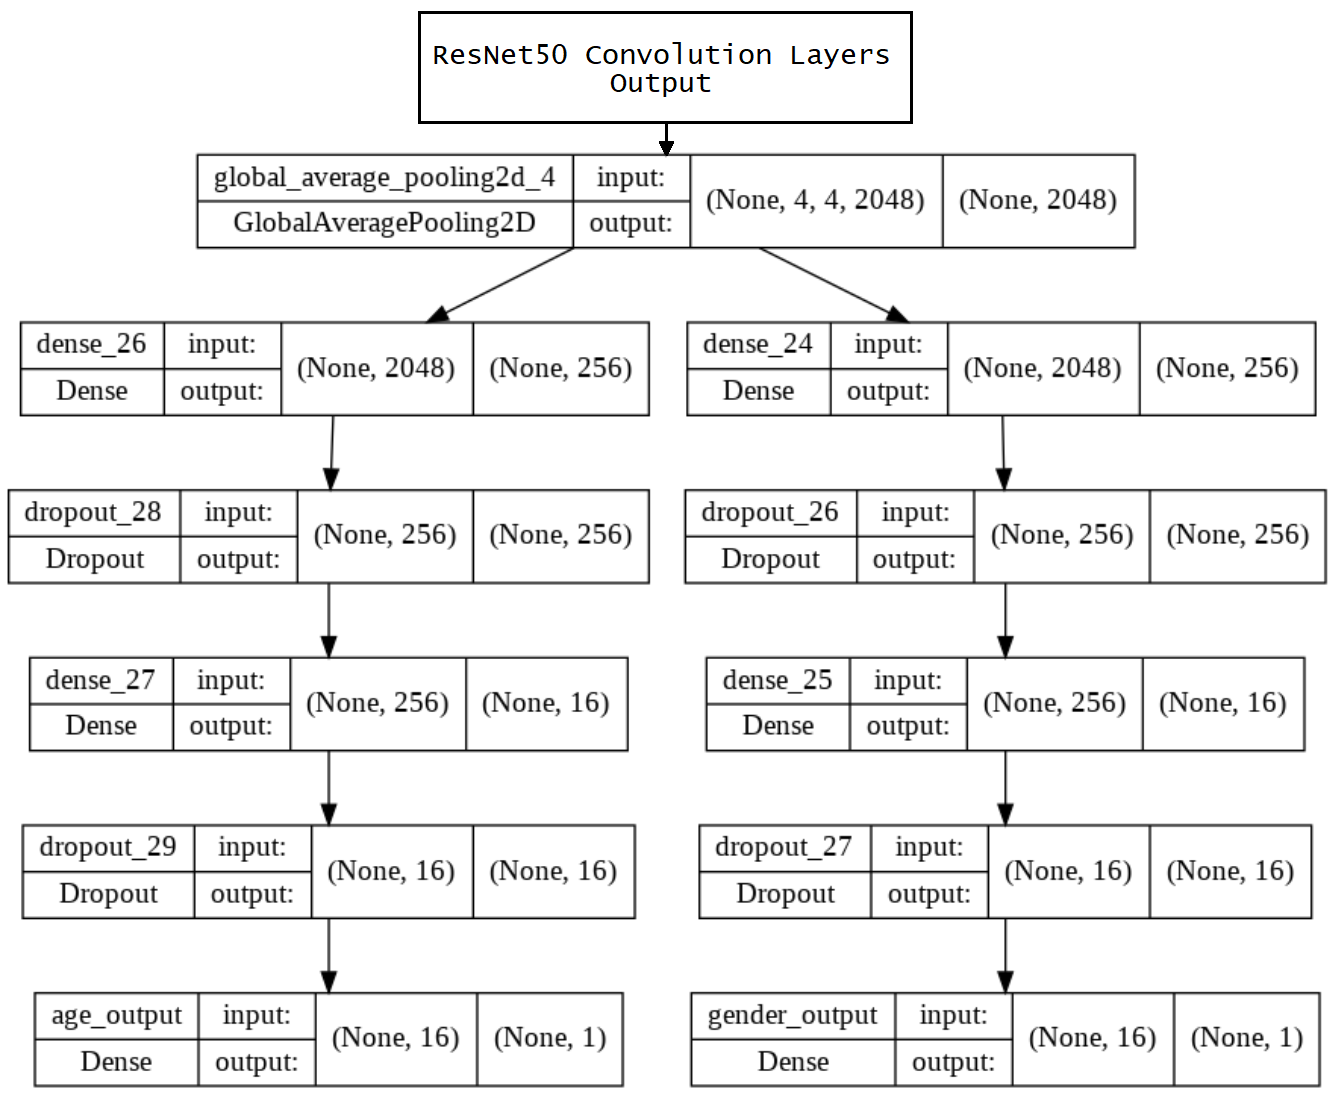
\includegraphics[height=0.5\textheight]{ModelBGraph_sample_simplified_dropouts_truncated.png}
\end{figure}

\subsection{Training}
The pre-trained model was trained in the same manner as Model A, with the same losses, loss weights, learning rate and optimizer. 

Unfortunately we found the model started heavily over-fitting after a number of epochs.\\
If left to train for longer it would continue to improve training accuracy, however validation would not, and occasionally get worse.
As a form of hyper-parameter training we implemented a stop early callback which would end the training and retain the best weights (with respect to validation loss output) if the validation loss failed to improve over 5 consecutive epochs.\\
The trace of the training when early stopping was performed can be found in \autoref{appendix:ModelB_early_stopping}, wherein there was no improvement in validation loss from epoch 26-30, and as such the model weights would be set to those obtained in epoch 25.

\subsubsection{Data Preparation}
The dataset was processed in the same manner as for training Model A.\\
An \verb|ImageDataGenerator| was created, and used to create a data generator for both training and validation images.

\begin{optional}
    \subsubsection{Hyper-Parameter Tuning}
    Hyper-Parameters were tuned in the same manner as for Model A.\\
    The difference being the hyper-parameters tuned were:
    \begin{enumerate}
        \item Initial Learning rate
        \item Flatten Vs Global Pooling: whether to flatten the 3D output from the final convolution layers to get a 1 x N*M*M (where N is the feature depth, and M is the kernel size), or to average across all the features to get a 1xN vector (N is the feature depth).
        \item Feature depth of final convolution layer (for both branches)
        \item Number of Units for first FCN layer (for both branches)
        \item Dropout rate (for both branches)
        \item Regularisation (for both branches)
    \end{enumerate}
    Once this completed, we rebuilt and trained the model with the tuned hyper-params fixed.\\
    \begin{notes}
        This could be thrown into a table in the appendix if we want to ref we did tuning without wasting space on the specific params?
    \end{notes}
\end{optional}


\subsection{Performance}
Due to the early stopping implemented for Model B's training, the final Epoch is not the one from which the weights will be saved.\\
They will in-fact be saved from Epoch 25, since it failed to improve on the validation loss for 5 subsequent Epochs.\\
From Epoch 25, we can see Model B got the following performance:
\begin{table}[h!]
    \centering
    \begin{tabular}[h]{r|l|l}
        \hline
        Metric & Training & Validation \\
        \hline
        Age Mean Absolute Error & 6.6296 & 6.4352 \\
        \hline
        Gender Binary Accuracy & 0.9495 & 0.8952 \\
        \hline
    \end{tabular}
    \caption{\label{tab:ModelB_Performance}}
\end{table}
For the full training output for epoch 25, please see \autoref{appendix:modelB_best_epoch}.
For the training output for the final epochs (from the best epoch till the last), please see \autoref{appendix:modelB_early_stopping_epochs}.

Looking at the learning curves (shown in \autoref{fig:ModelBPerformanceAge}) of the age MAE for Model B, you can see very little over-fitting, with both lines sticking very close together with some minor spikes from the validation curve.\\
Unfortunately the gender accuracy shown in \autoref{fig:ModelBPerformanceGender} highlights a not insignificant amount of over-fitting, where validation accuracy always being at least 2\% more than the training accuracy, and starting to diverge from ~epoch 10.\\
\textit{The graphs within \autoref{fig:ModelBPerformance} }\\

\begin{figure}[h!]
    \begin{subfigure}{\textwidth}
        \centering
        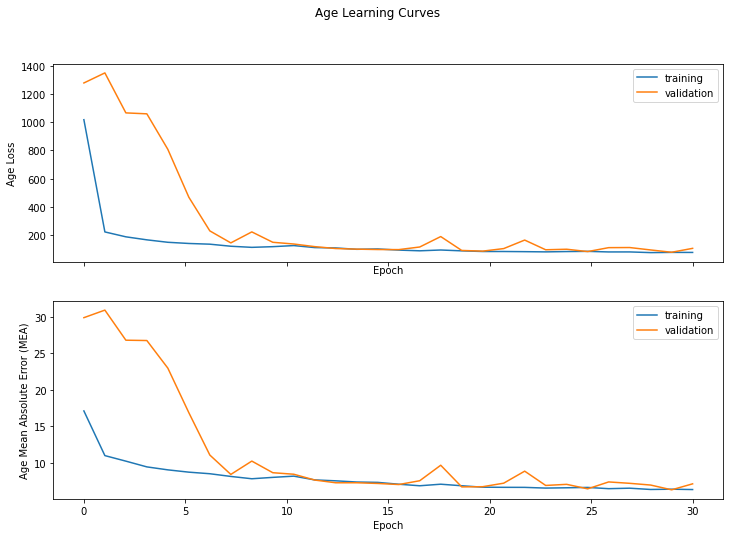
\includegraphics[height=0.45\textheight]{Model_B_AgeLearning_hp_tuned.png}
    \caption{\label{fig:ModelBPerformanceAge}The performance on age prediction for the pre-trained model.}
    \end{subfigure}
    \begin{subfigure}{\textwidth}
        \centering
        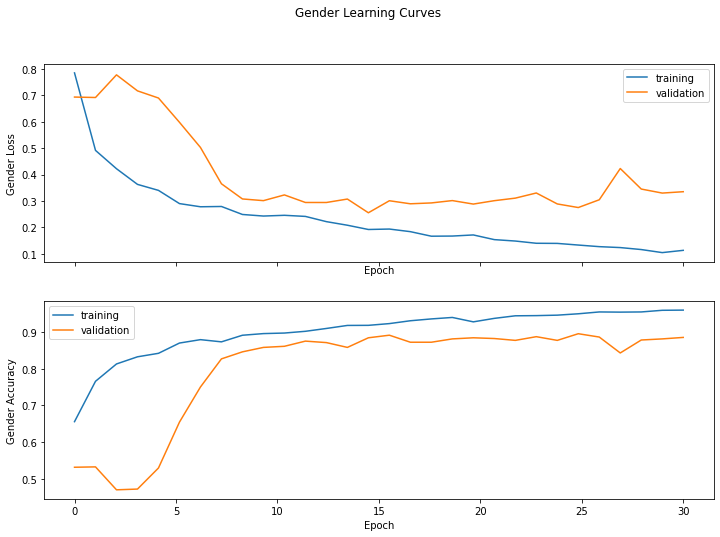
\includegraphics[height=0.45\textheight]{Model_B_GenderLearning_hp_tuned.png}
        \caption{\label{fig:ModelBPerformanceGender}The performance on gender prediction for the pre-trained model.}    
    \end{subfigure}
    \centering
    \caption{
        \label{fig:ModelBPerformance}Learning curves observed training Model B. \textit{Graphs show 30 epochs, however the weights are actually saved for epoch 25.}
        }
\end{figure}
